\section{Experimental Study}
\label{sec-expt}

%%%%%%%%%%%%%%%%%%%%%%%%%%%%%%%%%%%%%%%%%%%%%%%%%
\begin{figure*}[tb!]
%\begin{widepage}
%\vspace{-1.5ex}
\begin{center}
	
\subfigure[{\scriptsize Varying $|V_{P}|$ (\citationd)}]{\label{fig-exp-semantic-citation-diameter}
\includegraphics[scale=0.38]{./fig/citation-semantic-diameter.eps}}
\hspace{0.2ex}
\subfigure[{\scriptsize Varying $|V_{P}|$ (\citationd)}]{\label{fig-exp-semantic-citation-density}
\includegraphics[scale=0.38]{./fig/citation-semantic-density.eps}}
\hspace{0.2ex}
\subfigure[{\scriptsize Varying $|V_{P}|$ (\citationd)}]{\label{fig-exp-semantic-citation-capacity}
\includegraphics[scale=0.38]{./fig/citation-semantic-capacity.eps}}
\hspace{0.2ex}
\subfigure[{\scriptsize Varying $|V_{P}|$ (\citationd)}]{\label{fig-exp-semantic-citation-link}
\includegraphics[scale=0.38]{./fig/citation-semantic-link.eps}}
\vspace{-2.5ex}

\subfigure[{\scriptsize Varying $k$ (\citationd)}]{\label{fig-exp-semantic-citation-diameter-varyk}
\includegraphics[scale=0.38]{./fig/citation-semantic-diameter-varyk.eps}}
\hspace{0.2ex}
\subfigure[{\scriptsize Varying $k$ (\citationd)}]{\label{fig-exp-semantic-citation-density-varyk}
\includegraphics[scale=0.38]{./fig/citation-semantic-density-varyk.eps}}
\hspace{0.2ex}
\subfigure[{\scriptsize Varying $k$ (\citationd)}]{\label{fig-exp-semantic-citation-capacity-varyk}
\includegraphics[scale=0.38]{./fig/citation-semantic-capacity-varyk.eps}}
\hspace{0.2ex}
\subfigure[{\scriptsize Varying $k$ (\citationd)}]{\label{fig-exp-semantic-citation-link-varyk}
\includegraphics[scale=0.38]{./fig/citation-semantic-link-varyk.eps}}
\vspace{-2.0ex}
\end{center}

%\vspace{-2ex}
\vspace{-3ex}
\caption{Performance evaluation of algorithm \optgrouprec for top-$k$ team formation}
\label{exp-semantic-effectiveness-citation}
%\end{widepage}
\vspace{-3.0ex}
\end{figure*}

%We next present an experimental study using both real-life and synthetic data.
We conducted four sets of experiments to evaluate the performance of
(1) \optgrouprec for the top-$k$ team formation problem,
(2) \inc for the dynamic top-$k$ team formation problem
\wrt single sets of (a) pattern updates, (b) data updates, and (c) simultaneous pattern and data updates,
(3) \inc \wrt continuous sets of pattern and data updates, and
(4) the extra space cost of auxiliary structures used by \inc.


\subsection{Experimental Settings}

 We used the following real-life and synthetic datasets.

%\subsection{Experimental Settings}

\vspace{-0.3ex}
\etitle{Real-life graphs.} We used two real-life graphs.

\ni (1) {\em \citationd}~\cite{citationWeb} contains 1.39M paper nodes and 3.02M paper-paper citation edges.
We used its undirected version, where edges indicate the relevance relationship, and generated 200 labels based on phrase clustering of paper titles.

\ni (2) {\em \youtube}~\cite{youtubeWeb} contains 2.03M video nodes and 12.2M edges, which represent recommendations between two videos. We used the undirected version, and generated 400 labels based on the built-in categories and ages of videos.

\etitle{Synthetic graph generator.} We generated synthetic graphs (\synthetic) with community structures as existed in real-life, by adopting the LFR-benchmark graph model~\cite{AndreaSF08}. It is controlled by three parameters: the number $n$ of nodes, the average degree $d$ of nodes, and the number $l$ of node labels.



\eat{
 We used the following datasets and settings.	
	
\etitle{Data graphs.} We used two real-life and a synthetic datasets.

\ni (1) {\em \citationd}~\cite{citationWeb} is a real-life dataset containing 1.39M paper nodes and 3.02M paper-paper citation edges.
We used its undirected version, where edges indicate the relevance relationship. We generated 200 node labels based on phrase clustering of paper titles.

\ni (2) {\em \youtube}~\cite{youtubeWeb} contains 2.03M video nodes and 12.2M edges, which represent recommendations between two videos. We used the undirected version, and generated 400 labels based on the built-in categories and ages of videos.

\ni (3) We generated synthetic data graphs (\synthetic) with community structures as existed in real-life networks, by adopting the LFR-benchmark graph model~\cite{AndreaSF08}. It is controlled by three parameters: the number $n$ of nodes, the average degree $d$ of nodes, and the number $l$ of node labels.
%Given $n, d$, and $l$, the generator produces a graph with $n$ nodes, $n*d/2$ edges, and the nodes are labeled from a set of $l$ labels.

%\ni (3) We also used real-life dataset \youtube~\cite{youtubeWeb}. The detailed information of the dataset is available in the full version~\cite{fullvldb18}.
}%%%EAT

\etitle{Pattern generator}.
We implemented a generator to produce pattern graphs, controlled by 4 parameters:
the number of nodes $|V_P|$, the number of edges $|E_P|$, the label $l_{P}$ for each node from
an alphabet of labels in the corresponding data graphs,
and the capacity bound $f_{P}$ for each node.

\etitle{Algorithms}. We implemented the following algorithms, all in C++:
(1) algorithm \optgrouprec for \teamF, (2) incremental algorithm \inc for \dynteamF,
(3) three compared top-$k$ team formation algorithms \mindia, \minsumdis and \denalk, where
(a) \mindia is to minimize the team diameter~\cite{Lappas09}, which is firstly proposed for the team formation problem,
(b) \minsumdis is to minimize the sum of all-pair shortest distances of teams~\cite{Kargar11}, and
(c) \denalk is to maximize the team density~\cite{GajewarS12}, which has the same goal with our algorithms.
Most of the algorithms for \teamF, including  \mindia and \denalk, only compute the best team,
while \minsumdis is able to find top-$k$ teams in polynomial time, which is an adaption of Lawler's procedure \cite{Lawler1972}.
Based on this, we extend \mindia and \denalk to find top-$k$ teams in polynomial time.

We used a PC with Intel Core i5-4570 CPU and 16GB of memory. We randomly generated 3 sets of input and repeated 5 times for each test. The average is reported here.
%We also used another real-life dataset \youtube, which will be reported in the Appendix.

\subsection{Experimental Results}

We present our findings. In all the experiments, we set $k=10$, $r=2$, $h=3$, $(|V_{P}|,$ $|E_{P}|)$ to be (10,12),
and capacity bounds to be [1,10] by default.
When generating synthetic graphs, we fixed $n=10^7$, $d=10$ and $l=200$.
All the findings on \youtube are reported in the full version~\cite{fullvldb18}.


\stitle{Exp-1: Efficiency of \optgrouprec}. We firstly evaluated the efficiency of \optgrouprec vs. \mindia, \minsumdis and \denalk.
We generated pattern graphs for \optgrouprec, and the corresponding queries (labels requirements) for \mindia, \minsumdis and \denalk.

Algorithms \mindia, \minsumdis and \denalk do not scale well on large graphs.
Indeed,  (1) \mindia and \minsumdis took more than $8$ hours to finish their preprocessing, \ie computing all-pair-shortest-paths;
and (2) \denalk took more than 24 hours even when $k=1$ on \citationd.
By contrast, \optgrouprec took around 100 seconds on \citationd by default settings.
Hence, we report the effectiveness of these algorithms on a sampled data graph with $10,000$ nodes on \citationd only.
%We further evaluate the efficiency of \optgrouprec in the incremental experiments.


\stitle{Exp-2: Effectiveness of \optgrouprec}. We then evaluated the efficiency of \optgrouprec vs. \mindia, \minsumdis and \denalk by checking the quality of matches returned by them.

\eat{%%%
\etitle{(1) Case study.}
We find \optgrouprec is able to identify sensible matches meeting the practical requirements.
We illustrate this with a real-life example pattern graph.

As shown in Fig.~\ref{fig-exp-1-effect-citation}, pattern graph $P_C$ is to find
(a) a set of papers in \citationd that ``Databases'', ``Data Mining'' and ``Artificial Intelligence'' papers are related to each other;
(b) ``Data Mining'' papers are related to ``Software Engineering'' papers; and
(c) the required number of papers for each domain is shown on $P_C$.
In \citationd, nodes are papers with unique id from different domains,
with labels indicating their domains, and they only match the nodes of $P_C$
with the same geometry shapes, \ie circles, ellipses and squares.

The match result of $P_C$ is shown in Figure~\ref{fig-exp-1-effect-citation}.
Observe that subgraph $G_C$ is the top-1 match result found by \optgrouprec for $P_C$, but cannot be found by \mindia, \minsumdis and \denalk, while $G'_C$ and $G''_C$ are the top-1 results found by \mindia and \minsumdis respectively.
The top-1 result found by \denalk is the densest component composed of 819 nodes (omitted).
These tell us that \optgrouprec has more expressive power than the other team formation algorithms
by identifying sensible matches satisfying the structural and capacity requirements.}%%%EAT


To evaluate the quality of teams found by the above four algorithms for \teamF, we defined four quality measures.
Consider a matched subgraph $G_S$ and pattern $P(V_P, E_P)$.

\noindent {(a) [{\em Diameter}]}: the diameter of $G_S$.

\noindent {(b) [{\em Density}]}: the density of $G_S$.

\noindent {(c) [{\em Node satisfiability}]}: $\eta_V(G_S, P)$ = $\#\kw{sat}_V(G_S, P) / |V_P|$, where $\#\kw{sat}_V(G_S, P)$ is the number of nodes in $P$ that are satisfied by $G_S$, in which we say a pattern node $u$ is satisfied by $G_S$ if there are a set $V_u$ of nodes in $G_S$ that match $u$ and moreover, $V_u$ satisfies the capacity constraints on $u$.

\noindent {(d) [{\em Edge satisfiability}]}: $\eta_E(G_S, P)$ = $\#\kw{sat}_E(G_S,P)/|E_P|$, where $\#\kw{sat}_E(G_S,P)$ is the number of edges in $P$ satisfied by $G_S$, in which we say an edge $(u_1, u_2)$ is satisfied by $G_S$ if for each $v_1$ in $G_S$ that matches $u_1$,
there exists $(v_1, v_1')$ in $G_S$ so that $v_1'$ matches $u_2$, and for each  $v_2$ in $G_S$ that matches $u_2$, there exists $(v_2, v_2')$ in $G_S$ such that $v_2'$ matches $u_1$.
\looseness=-1


Note that (a) and (b) are two traditional quality measures utilized by existing team formation algorithms~\cite{GajewarS12,realTeamForm13,Lappas09,Kargar11}.
Intuitively, $\eta_V(G_S, P)$ (resp. $\eta_E(G_S,P)$) measures how well $G_S$ meets the node capacity requirements (resp. structural constraints) in $P$, and their values fall in $[0, 1]$.



\etitle{(i) Impacts of $|V_{P}|$}. Varying the number $|V_{P}|$ of
nodes in $P$ from 4 to 16, we took the average value of top-$k$ teams found by  \optgrouprec, \mindia, \minsumdis and \denalk \wrt four quality measures.
The results are reported in Figures \ref{fig-exp-semantic-citation-diameter}-\ref{fig-exp-semantic-citation-link}.

Observe the following.
(1) The diameters of teams found by \optgrouprec are comparable to those of \mindia and \minsumdis, which are in particularly designed to minimize the diameters, as shown in Fig.~\ref{fig-exp-semantic-citation-diameter}. This is ensured by the use of balls in \optgrouprec.
(2) The densities of teams found by \optgrouprec, though are smaller than \denalk which is specialized for maximizing team densities, are larger than \mindia and \minsumdis, as in Fig.~\ref{fig-exp-semantic-citation-density}.
(3) The node satisfiability of teams found by \optgrouprec is much higher than \mindia, \minsumdis and \denalk, \eg 1.0 vs. no larger than 0.2 in all cases as in Fig.~\ref{fig-exp-semantic-citation-capacity}.
(4) The teams found by \optgrouprec come with a higher edge satisfiability , \eg 1.0 in all cases, compared to smaller than 0.6 by \mindia, \minsumdis and \denalk, as shown in Fig.~\ref{fig-exp-semantic-citation-link}.

%%
%\revise{(1) In Fig.~\ref{fig-exp-semantic-citation-diameter}, the diameter of teams found by \optgrouprec is less than \mindia and \minsumdis, but the teams are with a small diameter, \eg less than \denalk, because of the ball restriction of \optgrouprec;}
%(2) in Fig.~\ref{fig-exp-semantic-citation-density}, the density of teams found by \optgrouprec is less than \denalk, while is higher than \mindia and \minsumdis;
%(3) in Fig.~\ref{fig-exp-semantic-citation-capacity}, the node satisfiability of teams found by \optgrouprec, \ie 1.0 in all cases, is much higher than \mindia, \minsumdis and \denalk, \ie less than 0.2; and
%(4) in Fig.~\ref{fig-exp-semantic-citation-link}, the teams found by \optgrouprec come with a higher edge satisfiability , \ie 1.0 in all cases, compared to less than 0.6 by \mindia, \minsumdis and \denalk.

\etitle{(ii) Impacts of $k$}. Varying $k$ from 1 to 20, we report the results in Figures
\ref{fig-exp-semantic-citation-diameter-varyk}-\ref{fig-exp-semantic-citation-link-varyk}.
Observe that the quality of teams found by the four algorithms shows the same rule as varying $|V_{P}|$, and the quality is not sensitive to $k$, a desirable property when top-$k$ semantics is concerned.

These verify that \optgrouprec can effectively preserve structural and capacity constraints for top-$k$ team formation \wrt edge and node satisfiability, and pertains a good team collaboration compatibility \wrt diameter and density.

\begin{figure*}[tb!]
%\begin{widepage}
\begin{center}
%\hspace{-5.5ex}
\subfigure[{\scriptsize Varying $|\Delta P|$ (deletions)}]{\label{fig-exp-patinc-del}
\includegraphics[scale=0.38]{./fig/union-pattern-deletion.eps}}
\hspace{0.2ex}
\subfigure[{\scriptsize Varying $|\Delta P|$ (insertions)}]{\label{fig-exp-patinc-ins}
\includegraphics[scale=0.38]{./fig/union-pattern-insertion.eps}}
\hspace{0.2ex}
\subfigure[{\scriptsize Varying $|\Delta P|$ (capacity)}]{\label{fig-exp-patinc-cap}
\includegraphics[scale=0.38]{./fig/union-pattern-capchange.eps}}
\hspace{0.2ex}
\subfigure[{\scriptsize Varying $|\Delta P|$ (hybrid updates)\hspace{-8.5ex}}]{\label{fig-exp-patinc-hyb}
\includegraphics[scale=0.38]{./fig/union-pattern-hybrid.eps}}
\vspace{-2.5ex}

%\hspace{-5.5ex}
\subfigure[{\scriptsize Varying $|\Delta G|$ (deletions)}]{\label{fig-exp-datainc-del}
\includegraphics[scale=0.38]{./fig/union-data-deletion.eps}}
\hspace{0.2ex}
\subfigure[{\scriptsize Varying $|\Delta G|$ (insertions)}]{\label{fig-exp-datainc-ins}
\includegraphics[scale=0.38]{./fig/union-data-insertion.eps}}
\hspace{0.2ex}
\subfigure[{\scriptsize Varying $|\Delta G|$ (hybrid updates)}\hspace{-5.5ex}]{\label{fig-exp-datainc-hyb}
\includegraphics[scale=0.38]{./fig/union-data-hybrid.eps}}
\hspace{0.2ex}
\subfigure[{\scriptsize Vary $(|\Delta P|,|\Delta G|)$ (simultaneous)}\hspace{-8.5ex}]{\label{fig-exp-hyb-patdata}
\includegraphics[scale=0.38]{./fig/union-pattern-data.eps}}
\vspace{-2.5ex}

%\hspace{-5.5ex}
\subfigure[{\scriptsize Varying $|\Delta P|$ in update sets}]{\label{fig-exp-patinc-multi}
\includegraphics[scale=0.38]{./fig/union-pattern-multi.eps}}
\hspace{0.2ex}
\subfigure[{\scriptsize Varying $|\Delta G|$ in update sets}]{\label{fig-exp-datainc-multi}
\includegraphics[scale=0.38]{./fig/union-data-multi.eps}}
\hspace{0.2ex}
\subfigure[{\scriptsize Vary $(|\Delta P|,|\Delta G|)$ in update sets}\hspace{-8.5ex}]{\label{fig-exp-hyb-datapat-multi}
\includegraphics[scale=0.38]{./fig/union-pattern-data-multi.eps}}
\hspace{0.2ex}
\subfigure[{\scriptsize Varying Datasets}]{\label{fig-exp-extraspace}
\includegraphics[scale=0.38]{./fig/union-space.eps}}
\vspace{-2ex}
\end{center}
\vspace{-2.5ex}
\caption{Performance evaluation of algorithm \inc for dynamic top-$k$ team formation (Cit: \citationd, Syn: \synthetic)}
\label{exp-inc}
%\end{widepage}
\vspace{-2.5ex}
\end{figure*}

\stitle{Exp-3: Efficiency of \inc for single set of updates}. We evaluated the efficiency of algorithm \inc for processing one set of pattern updates, data updates and simultaneous pattern and data updates vs. algorithm \optgrouprec on \citationd and \synthetic, respectively.


\etitle{(i) Pattern updates}. We fixed $(|V_{P}|,$ $|E_{P}|)$ to be $(10, 12)$, and varied the number $|\Delta P|$ of unit updates from 1 to 11, corresponding to 4.5\% to 49.5\% in
Figs. \ref{fig-exp-patinc-del}, \ref{fig-exp-patinc-ins}, \ref{fig-exp-patinc-cap} and \ref{fig-exp-patinc-hyb},
which show the results when $\Delta P$ contains (edge and node) deletions, (edge and node) insertions, capacity changes and hybrid pattern updates (5 types) respectively,
while keeping the proportion for each type equal.

We find the following.
(1) \inc outperforms \optgrouprec even when deletions are no more than 40.5\% on \citationd and 49.5\% on \synthetic;
%When the changes are no more than 27\%, \optinc improves \optgrouprec by over 50\% and 94\% on Citation and synthetic data, respectively.
\inc consistently does better than \optgrouprec due to the early-return strategy.
%This verifies the effectiveness of early-return strategy.
(2) \inc improves \optgrouprec to a large extent when only processes insertions and capacity changes.
(3) For the same $|\Delta P|$, \inc needs less time to process insertions than deletions.
%\eg it takes 26 seconds to handle 5 pattern deletions, but only 1 second to process insertions of the same size on Citation.
(4) When processes hybrid pattern updates, \inc outperforms \optgrouprec when changes are no more than (31.5\%, 40.5\%) on (\citationd, \synthetic);
%When the changes are no more than 27\%, \optinc improves \optgrouprec by over 33\% and 90\% on Citation and synthetic data, respectively.
%\inc takes more time than \optgrouprec when the changes are more than (36\%, 40.5\%) on (\citationd, \synthetic).
It is because all balls are identified as \affballsx when pattern updates accumulate to a certain extent.

\etitle{(ii) Data updates}. For (edge and node) deletions (resp. insertions) on datasets,
\eg\ \citationd with $|G|=4.4M$,
we varied $|G|$ from $4.4M$ to $2.22M$ (resp. from $3.05M$ to $4.4M$) in $4.5\%$ decrements (resp.\,$4\%$ increments) by randomly picking a subset of nodes and edges and removing from $G$ (resp. inserting into $G$);
For hybrid data updates (4 types), we randomly sampled a subgraph $G_s$ and removed from $G$, obtaining the initial $G$. %obtaining the initial $G$ with $|G|=3.66M$.
We varied $|G|$ by firstly removing a subset of nodes and edges from $G$ and then inserting a subset of nodes and edges from $G_s$ into $G$, in total  $4\%$ updates.
%The data updates generation method is same on synthetic data.
The results are shown in Figures \ref{fig-exp-datainc-del}, \ref{fig-exp-datainc-ins} and \ref{fig-exp-datainc-hyb}.

We find the following.
(1) \inc outperforms \optgrouprec when insertions are no more than 28\% and 32\% on \citationd and \synthetic (resp. 40.5\% and 45\% for deletions).
%When the changes are 16\% for insertions (resp. 20\% for deletions), \optinc improves \optgrouprec by over 42\% and 24\% (resp. 70\% and 91\%).
(2) For the same $|\Delta G|$, \inc needs less time to process deletions than insertions.
(3) We have conducted a survey: the user increment on Facebook~\cite{facebookStat} and Twitter~\cite{twitterStat} daily reaches 1.23\textperthousand\ and 2.47\textperthousand.
Therefore, \inc is able to handle the increments accumulated in dozens of days on Facebook and Twitter
at a high efficiency.
(4) \inc outperforms \optgrouprec when hybrid data updates are no more than 32\% and 36\% on \citationd and \synthetic, respectively.



\etitle{(iii) Simultaneous pattern and data updates}.  Varying the number of hybrid pattern updates from 1 to 7 and the amount of hybrid data updates from 4\% to 28\% together, corresponding to (4.5\%, 4\%) to (31.5\%, 28\%) for $(\Delta P, \Delta G)$ in Fig.~\ref{fig-exp-hyb-patdata}. We find that \inc outperforms \optgrouprec when $(\Delta P, \Delta G)$ is no more than (22.5\%, 20\%) and (27\%, 24\%) on \citationd and \synthetic, respectively.



\stitle{Exp-4: Efficiency of \inc for continuous sets of updates}. We evaluated \inc for a serial sets of pattern updates, data updates and simultaneous pattern and data updates vs. \optgrouprec on \citationd and \synthetic.


\etitle{(i) Pattern updates}. We generated $5$ sets of hybrid pattern updates, varying the number of updates in each set from $1$ to $7$.
We tested the average time took by \inc to finish all these sets one by one.
The results are reported in Fig.~\ref{fig-exp-patinc-multi}.

Recall that \inc adopts a lazy update policy, which definitely affects the processing time of next updates.
However, we find \inc outperforms \optgrouprec \wrt average time, when the amount of hybrid  pattern updates in each set is no more than (27\%, 31.5\%)  on (\citationd, \synthetic). This verifies the effectiveness of our lazy update policy.


\etitle{(ii) Data updates}. The setting is same as above. Varying the amount of hybrid data updates in each set from 4\% to 28\%,
the results are reported in Fig.~\ref{fig-exp-datainc-multi}.
We find that \inc outperforms \optgrouprec when hybrid data updates are no more than (24\%, 28\%) on (\citationd, \synthetic).



\etitle{(iii) Simultaneous pattern and data updates}. Using the same setting and varying the simultaneous pattern and data updates $(\Delta P, \Delta G)$ from (4.5\%, 4\%) to (31.5\%, 28\%) in Fig.~\ref{fig-exp-hyb-datapat-multi},
We find that \inc outperforms \optgrouprec when updates in each set are no more than (18\%, 16\%) and (22.5\%, 20\%)
on \citationd and \synthetic, respectively.
%\looseness=-1

\eat{%%%EAT
\begin{table}[h!]
%\vspace{-1ex}
\begin{center}
\begin{small}
%\vspace{-2ex}
\scriptsize
\begin{tabular}{|c|c|c|c|}
\hline
{\bf Datasets}       &  {\bf Auxiliary sizes}  &  {\bf Graph sizes}  &  {\bf Ratio} \\
\hline\hline
{\bf \citationd}            &  25MB       &        36MB    &     69.4\%   \\ \hline
{\bf \synthetic}       &  130MB       &        482MB      &     26.9\%   \\ \hline
\end{tabular}
\vspace{-1.5ex}
\end{small}
\caption{Extra space of auxiliary data structures}
\label{tab-extraspace}
\vspace{-5ex}
\end{center}
\end{table}
}%%%EAT

\stitle{Exp-5: Physical storage of auxiliary structures}. As shown in Fig.~\ref{fig-exp-extraspace}, the incremental algorithm \inc takes (25MB, 130MB) extra space to store all its auxiliary structures on (\citationd, \synthetic), while they need (36MB, 482MB) space to store themselves.
That is, the auxiliary structures are light-weight, and only take (69.4\%, 26.9\%) extra space compared with the original datasets.



%\begin{table}[h!]
%\vspace{-2ex}
%\vspace{2ex}
%\begin{center}
%\begin{small}
%%\vspace{-2ex}
%\scriptsize
%\begin{tabular}{|c|c|c|}
%\hline
%{\bf Storage}       &  {\bf Citation}  &  {\bf Synthetic}   \\
%\hline\hline
%{\bf Auxiliary}            &  25MB       &        130MB           \\ \hline
%{\bf Datasets}       &  36MB       &        482MB           \\ \hline
%{\bf Ratio}           &  69.4\%     &        26.9\%          \\ \hline
%\end{tabular}
%\vspace{-1.5ex}
%\end{small}
%\caption{Physical storage}
%\label{tab-notation}
%%\vspace{-7.5ex}
%\end{center}
%\end{table}


\stitle{Summary}. From these tests, we find the following.

\sstab(1) Our graph pattern matching approach is effective at capturing the practical requirements of top-$k$ team formation.

\sstab(2) Our batch algorithm for  top-$k$ team formation is efficient,
\eg it only took 116s when $|V|=1.39M$ and $|V_P|=10$.

\sstab (3) Our incremental algorithm for dynamic top-$k$ team formation is able to process continuous pattern and data updates, separately and simultaneously,
and it is more promising than its batch counterpart,
even (a) when changes are 36\% for pattern updates, 34\% for data updates, and (25\%, 22\%) for simultaneous pattern and data updates on average,
and (b) when 29\% for continuous pattern updates, 26\% for continuous data updates and (20\%, 18\%) for continuously simultaneous pattern and data updates on average.
